
The state of the art in breast finite element modeling was provided previously. Three models were identified representing the cutting-edge technologies in the field. The authors used prone MRI to estimate the breast reference geometry. The patient-specific constitutive parameters are chosen such that the best fit between the supine configuration estimate and the corresponding measured breast geometry is obtained. The models were evaluated using the measured and the estimated positions of superficial fiducial landmarks or internal anatomical landmarks in the supine breast configuration. As the optimization and evaluation  processes are based on the same data, the model limitations may by underestimated. For a better assessment of the model accuracy the evaluation on a third breast configuration is suitable.

 This chapter introduces a new biomechanical model developed by combining the best practices and concepts proved by previous works. To be as realistic as possible, our model considered breast heterogeneity, sliding boundary conditions, initial pre-stresses and personalized hyper-elastic properties of breast tissue. In addition, new types of soft tissue were included representing the breast support matrix composed of suspensory ligaments and fascias. Moreover, our model was built using prone and supine breast configurations and was evaluated in supine tilted configuration (\~ 45 deg) of the same volunteer.

In the first part of this chapter the data acquisition protocol is described and details on numerical methods and softwares used to extract the patient-specific breast geometry are given. Next, the different components of the finite element mesh are presented and the mesh quality is assessed using shape parameters.  Then, the assumptions on boundary conditions and materials models are explained. Finally, the model optimization process is detailed and results on patient-specific parameters and breast reference configuration are presented.   
\clearpage
\section{Geometry extraction}\label{section:geometryextraction}

Geometry extraction is the first step in FE analysis, and it
consists of obtaining the 3D surfaces of the
breast. We use the MR images to obtain the patient-specific breast volumes and the surrounding soft tissues distribution. Prior to surface extraction, the MRI volume is segmented and mapped to a single reference system. The next section describes the imaging acquisition protocol and the numerical method used to generate the 3D patient-specific breast geometry.

\subsection{Data acquisition}\label{subsection:imageaquisition}

 The images were acquired with a Siemens 3T scanner with T2 weighted image sequences. The in-plane image resolution was $0.5$x$0.5$ mm, and the slice thickness was 0.6 mm. During this acquisition, the contact between the breasts and the contours of the  relatively narrow MRI scanner tunnel, or with the patient body (arms, thorax), was minimized. Three different positioning configurations are considered: prone, supine and supine titled (\~ 45 deg). These positions were chosen to assess the largest possible deformations
\begin{figure}[H]
\centering
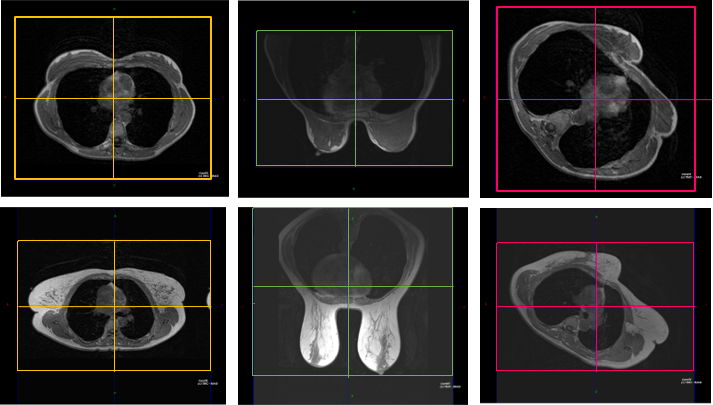
\includegraphics[width=0.9\textwidth,keepaspectratio]{figures/patientData.png} 
\caption{MRI images in three breast configuration: first line- subject 1; second line- subject 2}\label{fig:patientdata}
\end{figure}

Two volunteers agreed to participate in a pilot study approved by an ethical committee (MammoBio MAP-VS pilot study). The volunteers are 59 and 58 years old and have A-cup (subject 1) and F-cup (subject 2) breast size respectively. 
 

The volunteers were also asked to provide the compression force and breast thickness as measured on their most recent mammograms. Such data are summarized in Table \ref{tab:forceandthichnessdata}.
\begin{table}[H]
\centering
\begin{tabular}{c|c|c||c|c|}
\cline{2-5}
&\multicolumn{2}{c||}{Subject 1}&\multicolumn{2}{c|}{Subject 2}\\
\cline{2-5}
& Right breast & Left breast & Right breast & Left breast\\
\cline{2-5}
\hline
\multicolumn{1}{|c||}{Force (N)}  & 21.9 &40.9 &94.8 & 56.6 \\
\hline
\multicolumn{1}{|c||}{ Breast thickness (mm)} & 47 & 42 & 50 & 49 \\
\hline

\end{tabular}
\caption{Compression force and breast thickness for both subjects for a cranio-caudal mammogram}\label{tab:forceandthichnessdata}
\end{table}

\subsection{Image segmentation}%\label{subsection:imagesegmentation}

A semi-automated active contour method proposed by ITK-Snap software was used to segment the pectoral muscle and the breast tissues from MR images \citep{yushkevich_user_2006}. The segmentation process for one tissue type is performed progressively by small regions of interest (ROI, see Figure \ref{fig:breasttissuessegmentation}.a). For each ROI the segmentation of one tissue takes place in 3 steps (Figure \ref{fig:breasttissuessegmentation}):
\begin{enumerate}
\item Firstly, the random forest algorithm \citep{ho_random_1995} is used to compute a new synthetic volume consisting of the probability of each pixel to belong or not to the segmented tissue. The training data set is manually selected by the user and include state and space characteristics such as voxel grey intensity, voxel's neighbors intensity (with variable radius of neighboring) and voxel position (x; y; z) (Figure \ref{fig:breasttissuessegmentation}.c ). 

\item Secondly, spherical seeds point with variable radius are placed on the new synthetic volume to mark the connected components bellowing to the segmented tissue (Figure \ref{fig:breasttissuessegmentation}.d).
\item Finally, the placed seed point will evolve in the 3D space with a speed and direction derived from the pixel intensity and sign in the synthetic volume (Figure \ref{fig:breasttissuessegmentation}.d).
\end{enumerate}

 
 \begin{figure}[H]
\centering
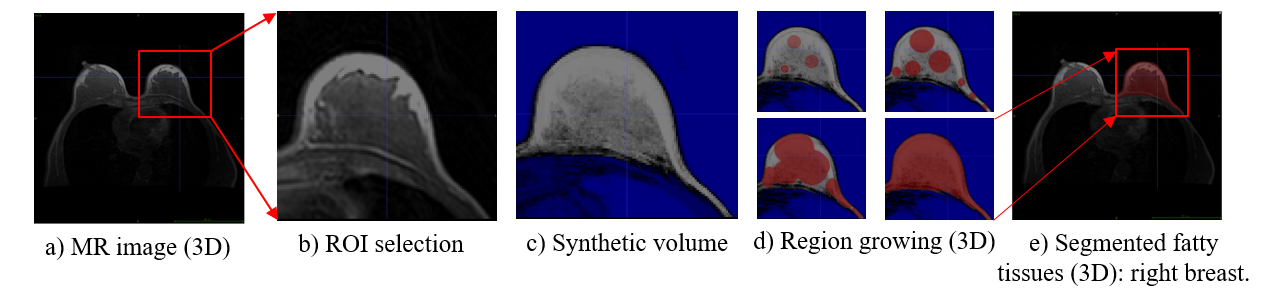
\includegraphics[width=1\textwidth,keepaspectratio]{figures/tissues_segmentation.png} 
\caption{Breast tissues segmentation on the breast MRI of the second volunteer. Prone breast configuration. White voxel - the voxel belongs to breast tissue ; blue voxel - the voxel don't belongs to fatty tissue} \label{fig:breasttissuessegmentation}
\end{figure}

 After segmentation, an additional manual correction was performed to refine components boundaries. Simple erosion and dilatation operations were applied on breast and muscle segmented volumes in order to obtain smoother connected components. Then, to avoid tissues overlapping at muscle-breast juncture border binary operations were used.
 
The process was repeated for both volunteers and for each breast configuration: supine, prone and supine tilted. The extracted surfaces in supine and prone configurations are used for model definition and optimization,  the last surface, in supine tilted configuration, is used for model evaluation. 

\subsection{Image registration}\label{subsection:image registration}

During the imaging acquisition process, the subject is moved in and outside the MRI scanner tunnel. Therefore, the breast not only undergoes an elastic deformation, but also a rigid transformation. Prior to image acquisition, four landmarks are fixed on the chest wall.  The landmarks are placed on sternum and inframammary fold lines; these regions are indeed known to be rich in fibrous ligaments limiting the soft tissue elastic deformation.  To assess the body position changes, a rigid transform is computed by minimizing the Euclidian distance between the two configurations of the four points defined by the four landmarks. The transformation is estimated using the iterative closest point (ICP) algorithm proposed by ITK library.

However, because of the small local deformations of skin soft tissues in the chest wall region, the computed rigid transformation is not accurate enough. Therefore, a second registration step is performed by aligning the bone structures of the anterior part of thoracic cage from prone and supine tilted positions to the supine one. The muscular tissues mask previously segmented are used in order to remove body soft tissues. The image registration is implemented using the gradient descent based algorithm minimizing the images cross correlation (ITK library).

Figure \ref{fig:patientdataregistered} shows overlapping  prone-supine and supine tilted-supine breast images in the transversal plane after registration. The anterior part of the chest line is well aligned, however there are some differences because of elastic thoracic cage deformations due to hand positions or body-mass force repartition. 

\begin{figure}[!h]
\centering
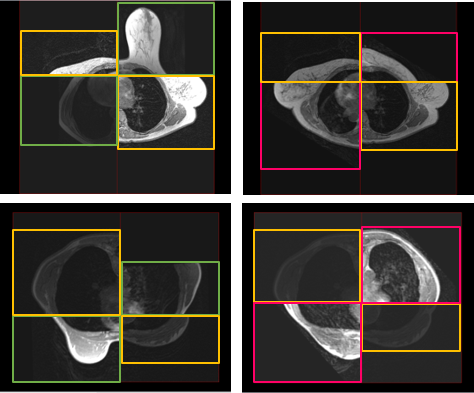
\includegraphics[width=0.7\textwidth,keepaspectratio]{figures/patientDataRegistered.png} 
\caption{Registered MRI images: first line- subject 1; second line- subject 2; first column - prone configuration versus supine; second column - supine tilted versus supine }\label{fig:patientdataregistered}
\end{figure}

In a multi-gravity loading finite element simulation, the gravity force is applied to the whole model as a body force. The gravity force orientation can be broken down into three components of the Cartesian coordinate system labeled X, Y, and Z directions (Figure \ref{fig:xyz_axis_directions}). The supine configuration was chosen as a reference state, therefore the gravity loading direction was set in that configuration to be oriented on the inverse direction of the Y axis (posterio-anterior direction, Figure \ref{fig:xyz_axis_directions}): $\gamma_s = (0,-1,0)$.   The gravity loading direction for the two other positions are given by the rigid transformation computed by images registration: $\gamma_p = (0.037, 0.985, -0.165)$ direction vector for gravity in prone position and $\gamma_{st} = (-0.744 , -0.667, 0.023)$ direction vector for supine tilted position for the second volunteer.

\begin{figure}[!ht]
\centering
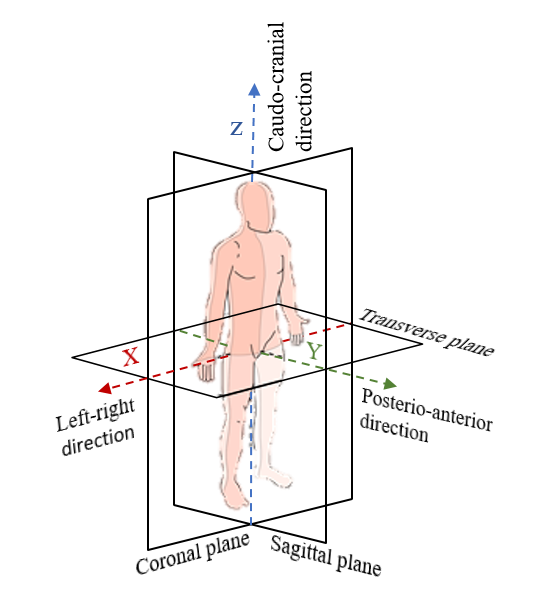
\includegraphics[width=0.45\textwidth,keepaspectratio]{figures/xyz_axis_directions.png} 
\caption{Anatomical planes and nominal Cartesian axis directions.}\label{fig:xyz_axis_directions}
\end{figure}

\subsection{Patient-specific 3D geometry}\label{subsection:patientspecificgeometry}

The breast patient-specific geometry was created based on the MR images in supine configuration. Following image segmentation (Figure \ref{fig:3dgeometries}.b), the outer shape of labeled regions are subsequently discretized by 2D triangular elements.  We used the semi-automatic Skin Surface module proposed by SpaceClaim Direct Modeler to convert the mesh surfaces to non-uniform rational basis spline (NURBS) surfaces (Figure \ref{fig:3dgeometries}.c). 

\begin{figure}[!h]
\centering
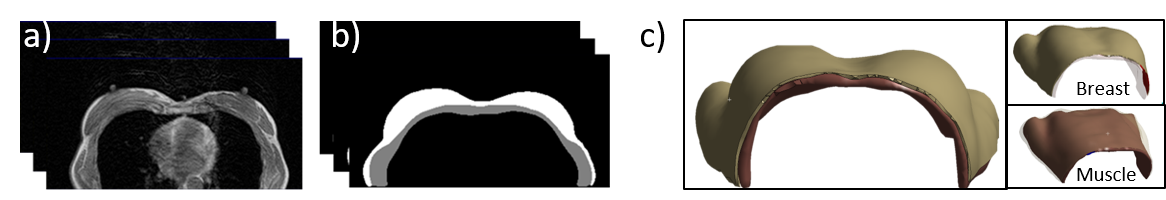
\includegraphics[width=\textwidth,keepaspectratio]{figures/3dgeometries.png} 
\caption{3D geometries generation. a) MR images; b) segmeted image; c) corresponding 3D geometries} \label{fig:3dgeometries}
\end{figure}

The NURBS are averaging curves between points, therefore they are smoother and easier to use in mechanical applications. Figure \ref{fig:nurbsVSsurfaceMeshError} shows the distance from the mesh surface to the NURBS surface for the breast and muscle geometries. The NURBS surface fits nearly all over the initial geometry within a tolerance of $0.5\ mm$. In areas with large curvature angles, the distance between the two surfaces increase up to $1.6\ mm$ and $3.06\ mm$ for breast and muscle geometries respectively.
 


\begin{figure}[!h]
\centering
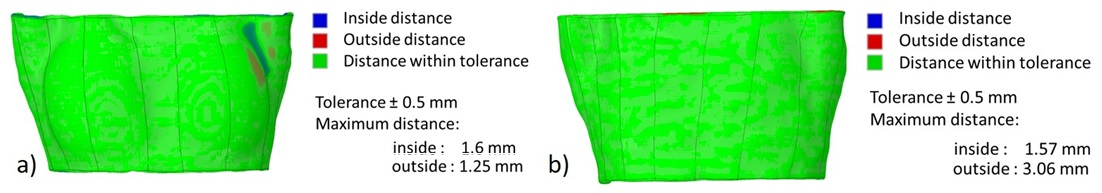
\includegraphics[width=\textwidth,keepaspectratio]{figures/nurbsVSsurfaceMeshError.jpg} 
\caption{Error betweeen the surface mesh surface and NURBS surface. a) Breast volume; b) muscle volume;} \label{fig:nurbsVSsurfaceMeshError}
\end{figure}


\section{ Finite Elements Mesh}\label{section:myFEM}

After computing the NURBS surfaces, the internal spatial information needs to be encoded using a volumetric mesh. The optimal elements type or mesh density in the simulation of FE models is still an open question and topic of debate. The use of hexahedral elements is usually assumed to result in a more accurate solution, especially when expecting high strain/stress gradients. However, in the literature, because of the large computational time, such meshes are used mostly with a reduced number of elements \citep{ruiter_model_based_2006,gamage_modelling_2012}. Tetrahedral elements are widely used due to their geometrical flexibility and because they provide a good trade-off between computation time and displacement accuracy \citep{han_nonlinear_2014,palomar_finite_2008,griesenauer_breast_2017}.   

In our case, an iterative optimization process is being considered to estimate the constitutive parameters. Therefore, to reduce the computation time, only linear tetrahedral elements are used. The first order elements are known to bear volumetric locking problems when used to model large strain for quasi-incompressible materials, \citep{fung_classical_2017}. When volumetric locking occurs, the displacements calculated by the finite element method are orders of magnitude smaller than they should be. It has been shown that a linear element with a mixed U-P formulation can avoid these problems \citep{rohan_finite_2014}. Therefore, in our work, the geometries are meshed using the solid element solid285 (ANSYS Mechanical) which provides a mixed U-P formulation option. 

 On the other hand, the mesh density has also an impact on model accuracy, a finer mesh resulting in a more accurate and stable solution, but also increasing the computational time. To our knowledge, no studies have determined the optimal resolution of the volumetric mesh for simulating breast tissues deformations. To determinate the appropriate mesh size, a mesh convergence study was performed. The details can be found in Appendix \ref{appendice:meshconvergence}.  According to these results the optimal element’s sizes range between 7 and 10mm. The mesh that was chosen for the second volunteer thus consists in 18453 tetrahedral elements with 9625 elements assigned to the pectoral muscle and the thoracic cage and 8828 elements assigned to breast tissues (Figure \ref{fig:meshcomponents}).
 
 \begin{figure}[!h]
\centering
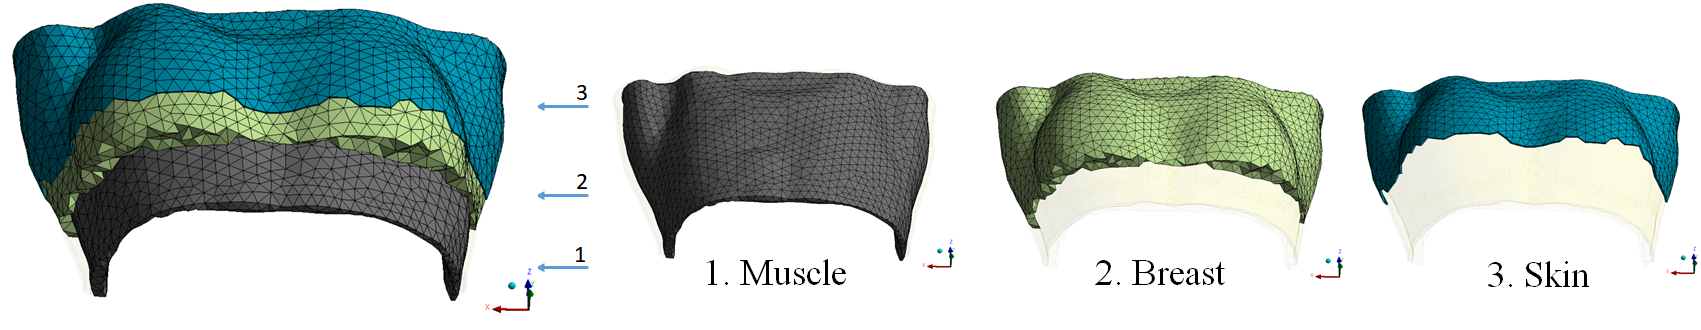
\includegraphics[width=1\textwidth,keepaspectratio]{figures/mesh3components.png} 
\caption{ Finite element mesh components. The tissues components are cropped for visualization purposes. }\label{fig:meshcomponents}
\end{figure}
 
 The mesh quality is measured using three criteria: element skewness, aspect ratio and maximal corner angle. The Figure \ref{fig:meshquality} shows the ranges of values for these shape parameters. The element's aspect ratio and maximal corner angle range between the nominal limits defining a good mesh quality (Section \ref{section:lagrangianmesh}). There is a small number of elements with a skewness lager than the maximal theoretical quality limit ( 0.75 ) , however there are no degenerated elements (skewness = 1).  

\begin{figure}[!h]
\centering
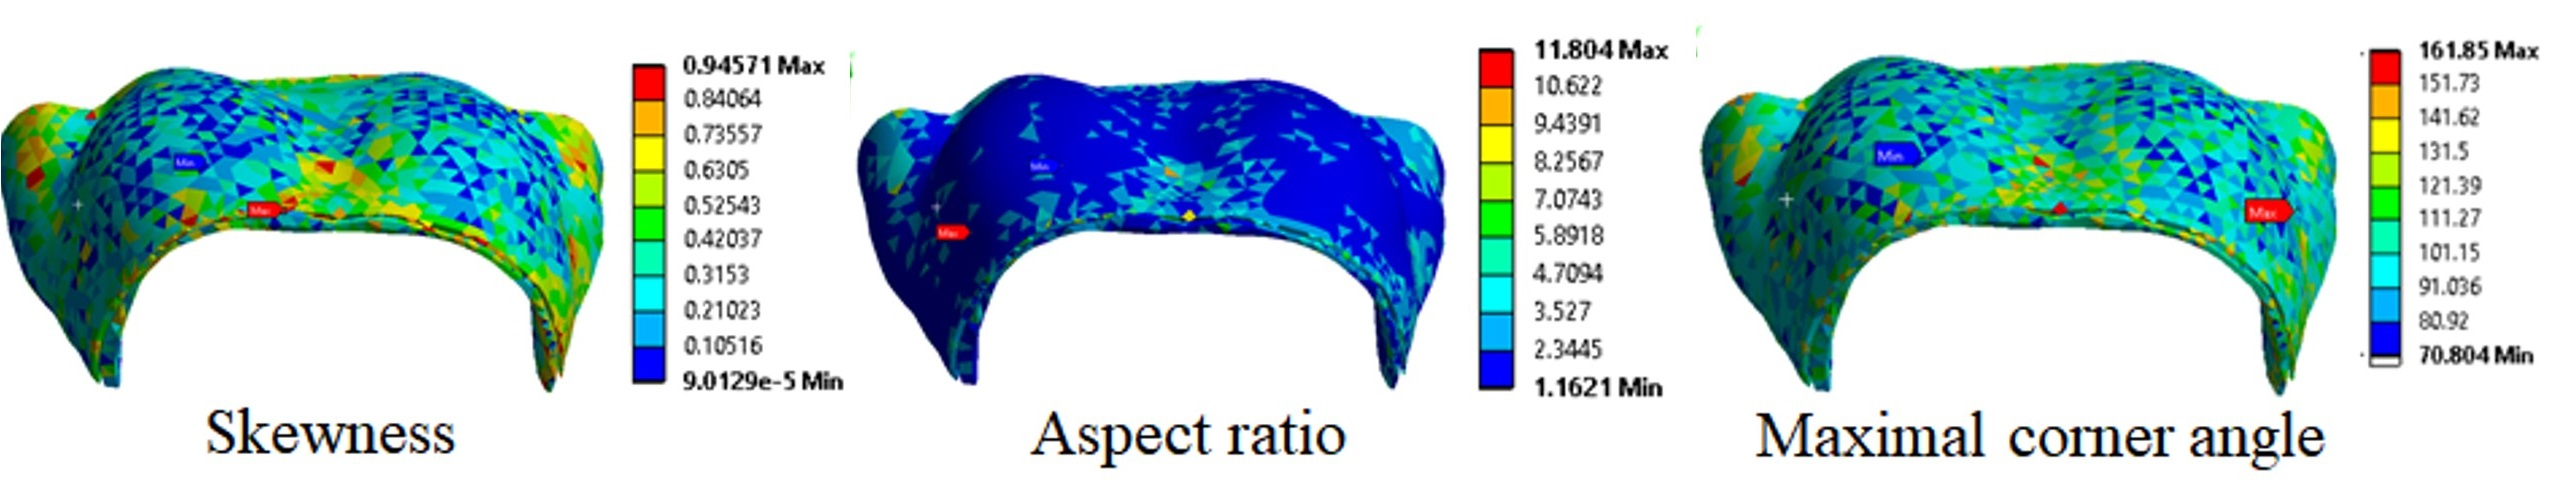
\includegraphics[width=1\textwidth,keepaspectratio]{figures/meshquality.jpg} 
\caption{ Finite elements mesh quality.}\label{fig:meshquality}
\end{figure}




The breast skin layer is added a posteriori   as a $2mm$ thick single layer of shell elements (1980 elements). Shell elements and the underlying solid elements are sharing the same nodes (Figure \ref{fig:meshquality}.a).



\section{Breast reference configuration}\label{section:myStressFree}
To estimate the reference configuration of the breast (\textit{stress-free} configuration), an adapted prediction-correction iterative approach was implemented \citep{eiben_breast_2014} using prone and supine image data sets. The overall iterative process is presented in Figure \ref{fig:myfixedpointalgo}. The first estimate of stress-free breast configuration is computed by applying an inverse gravity on the supine geometry. Then, at each iteration, the estimated stress-free configuration is used to simulate breast deformation due to gravity in a prone position. The differences between result of this simulation and the real shape of the breast in prone position is quantified by computing the Euclidian distances $D_i$ between the \textit{active nodes} defined at the breast external surface. These distances are then used in the next iteration of the process to simulate imposed displacements (Dirichlet condition) to the active nodes i in the stress-free configuration. To limit any mesh distortion, the displacements are only partially imposed using a multiplicative regularization factor $ (\alpha <1)$ \nomenclature{$\alpha$}{Multiplicative regularization factor}. The process repeats as long as the new transformation improves the similarity between the two geometries in prone configuration by more than $1mm$ on average. The similarity between the estimated and measured configurations is given by the mean Euclidean distance over the active nodes.                                                              

\begin{figure}[!h]
\centering
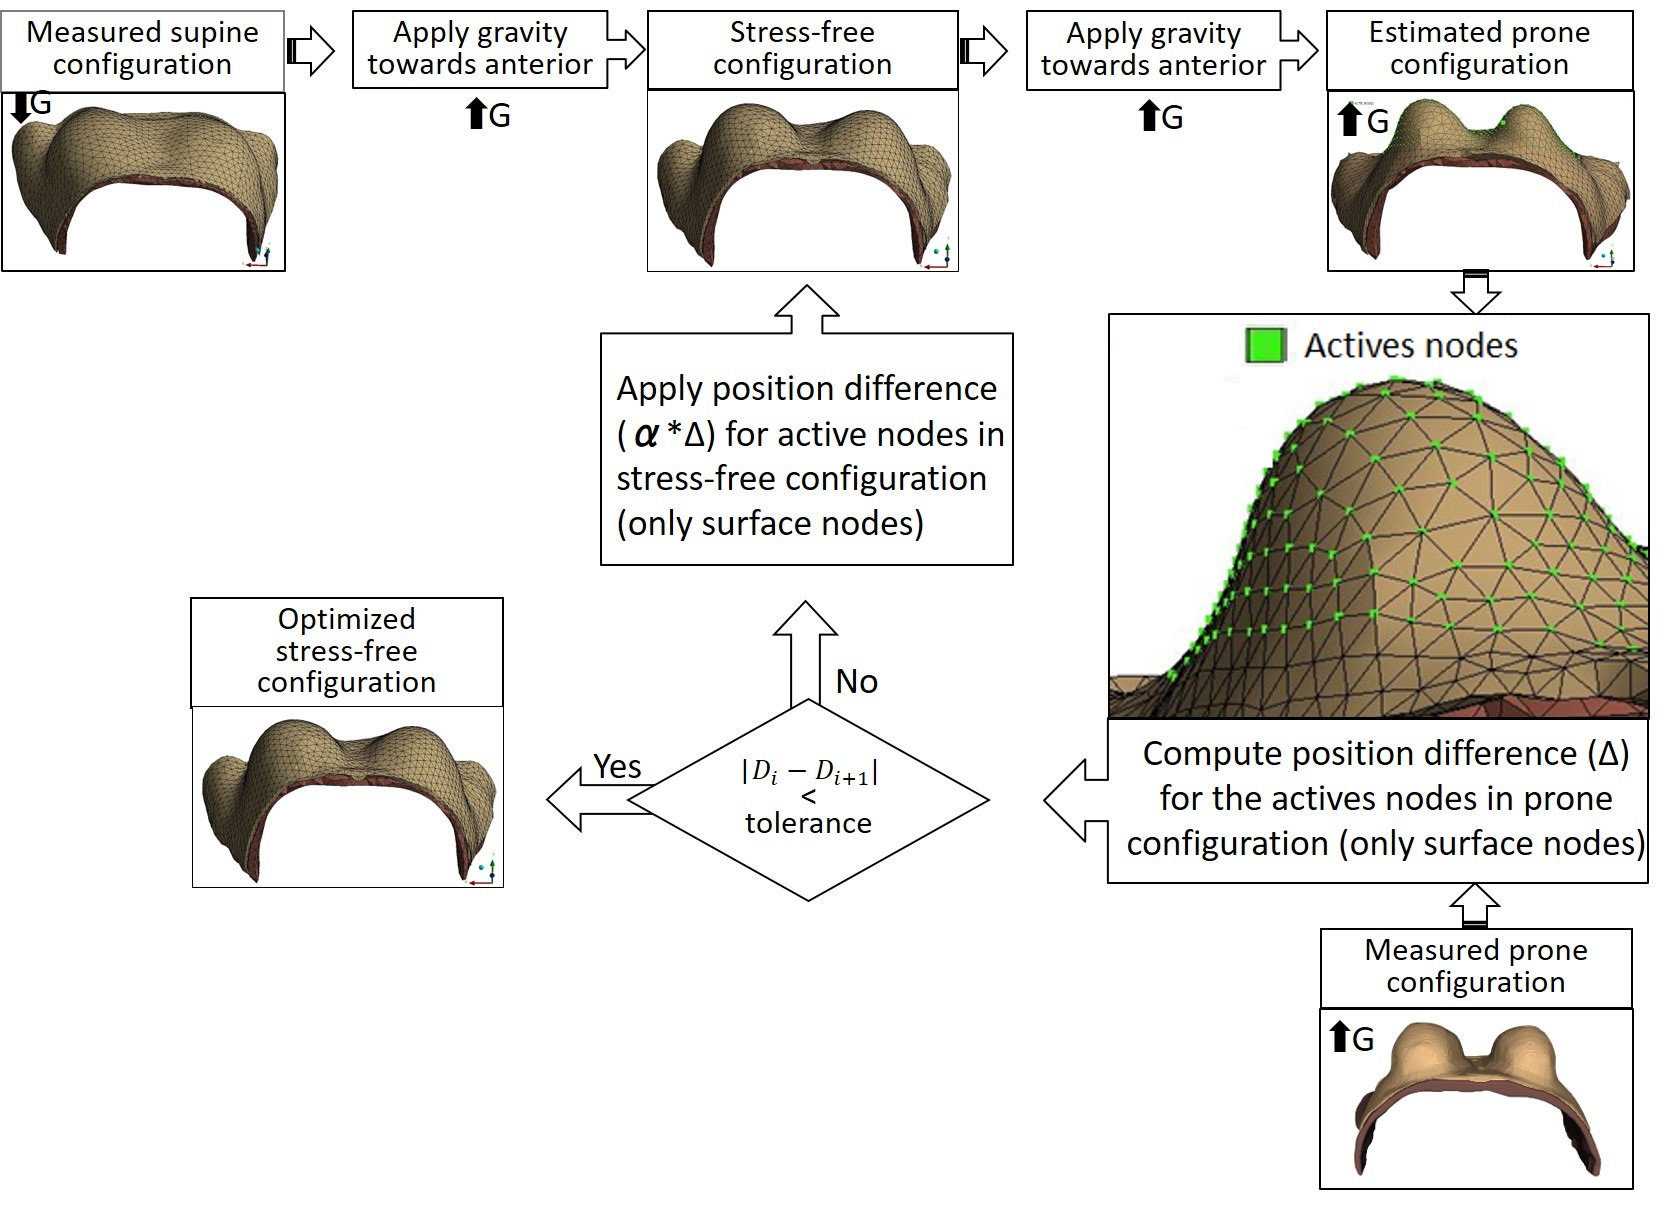
\includegraphics[width=0.9\textwidth,keepaspectratio]{figures/stress_free_config_algo.jpg} 
\caption{Fixed point type iterative algorithm for stress-free geometry approximation. $D_i$ - mean node to node distance over the active nodes at iteration $i$, $G$ - gravity force}\label{fig:myfixedpointalgo}
\end{figure}

During fitting process, the active nodes are chosen to be the ones corresponding only to the breast surface. The skin nodes bellowing to the  arms and the lateral thoracic areas are excluded  in order to neglect as much as possible the error due to rigid body changes.

To compute the position difference $D_i$ of the nodes $i$ between the estimated and the measured breast configurations\nomenclature{$D_i$}{Position difference of the node $i$ between the estimated and measured breast prone configurations}, the  positions of the active surface nodes on prone configuration have to be known. Thus, an additional mesh registration step is performed at each iteration: the active nodes are morphed into prone configuration using the elastic deformation method proposed by \cite{bucki_fast_2010}. The method estimates a C1-diffeomorphic, non-folding and one-to-one transformation to register a source point cloud onto a target data set D, which can either be a point cloud or a surface mesh.  The input source points set is initially embedded in a deformable virtual hexahedral elastic grid. Then an iterative registration technique is performed by successive elementary grid deformations and at different grid refinement levels. 


\section{Boundary conditions}\label{section:myBoundayconditions}

Breast deformations can be modeled by solving the
motion equations using two different types of boundary
conditions, regarding either displacements (Dirichlet conditions) or forces (Neumann conditions).

First, to provide a rigid support for the muscle mesh component, zero displacement conditions are imposed to its posterior face, assumed to be attached to the rib cage (figure \ref{fig:meshboundaries}). Next, the interface between the breast mesh and muscle mesh is models using contact mechanics. The muscle is stiffer than the adipose tissues, thus it's anterior face represents the target surface and the posterior breast face represents the contact surface (see Section \ref{section:contactmechanics} for a reminder of these target and source surfaces). 

\begin{figure}[!h]
\centering
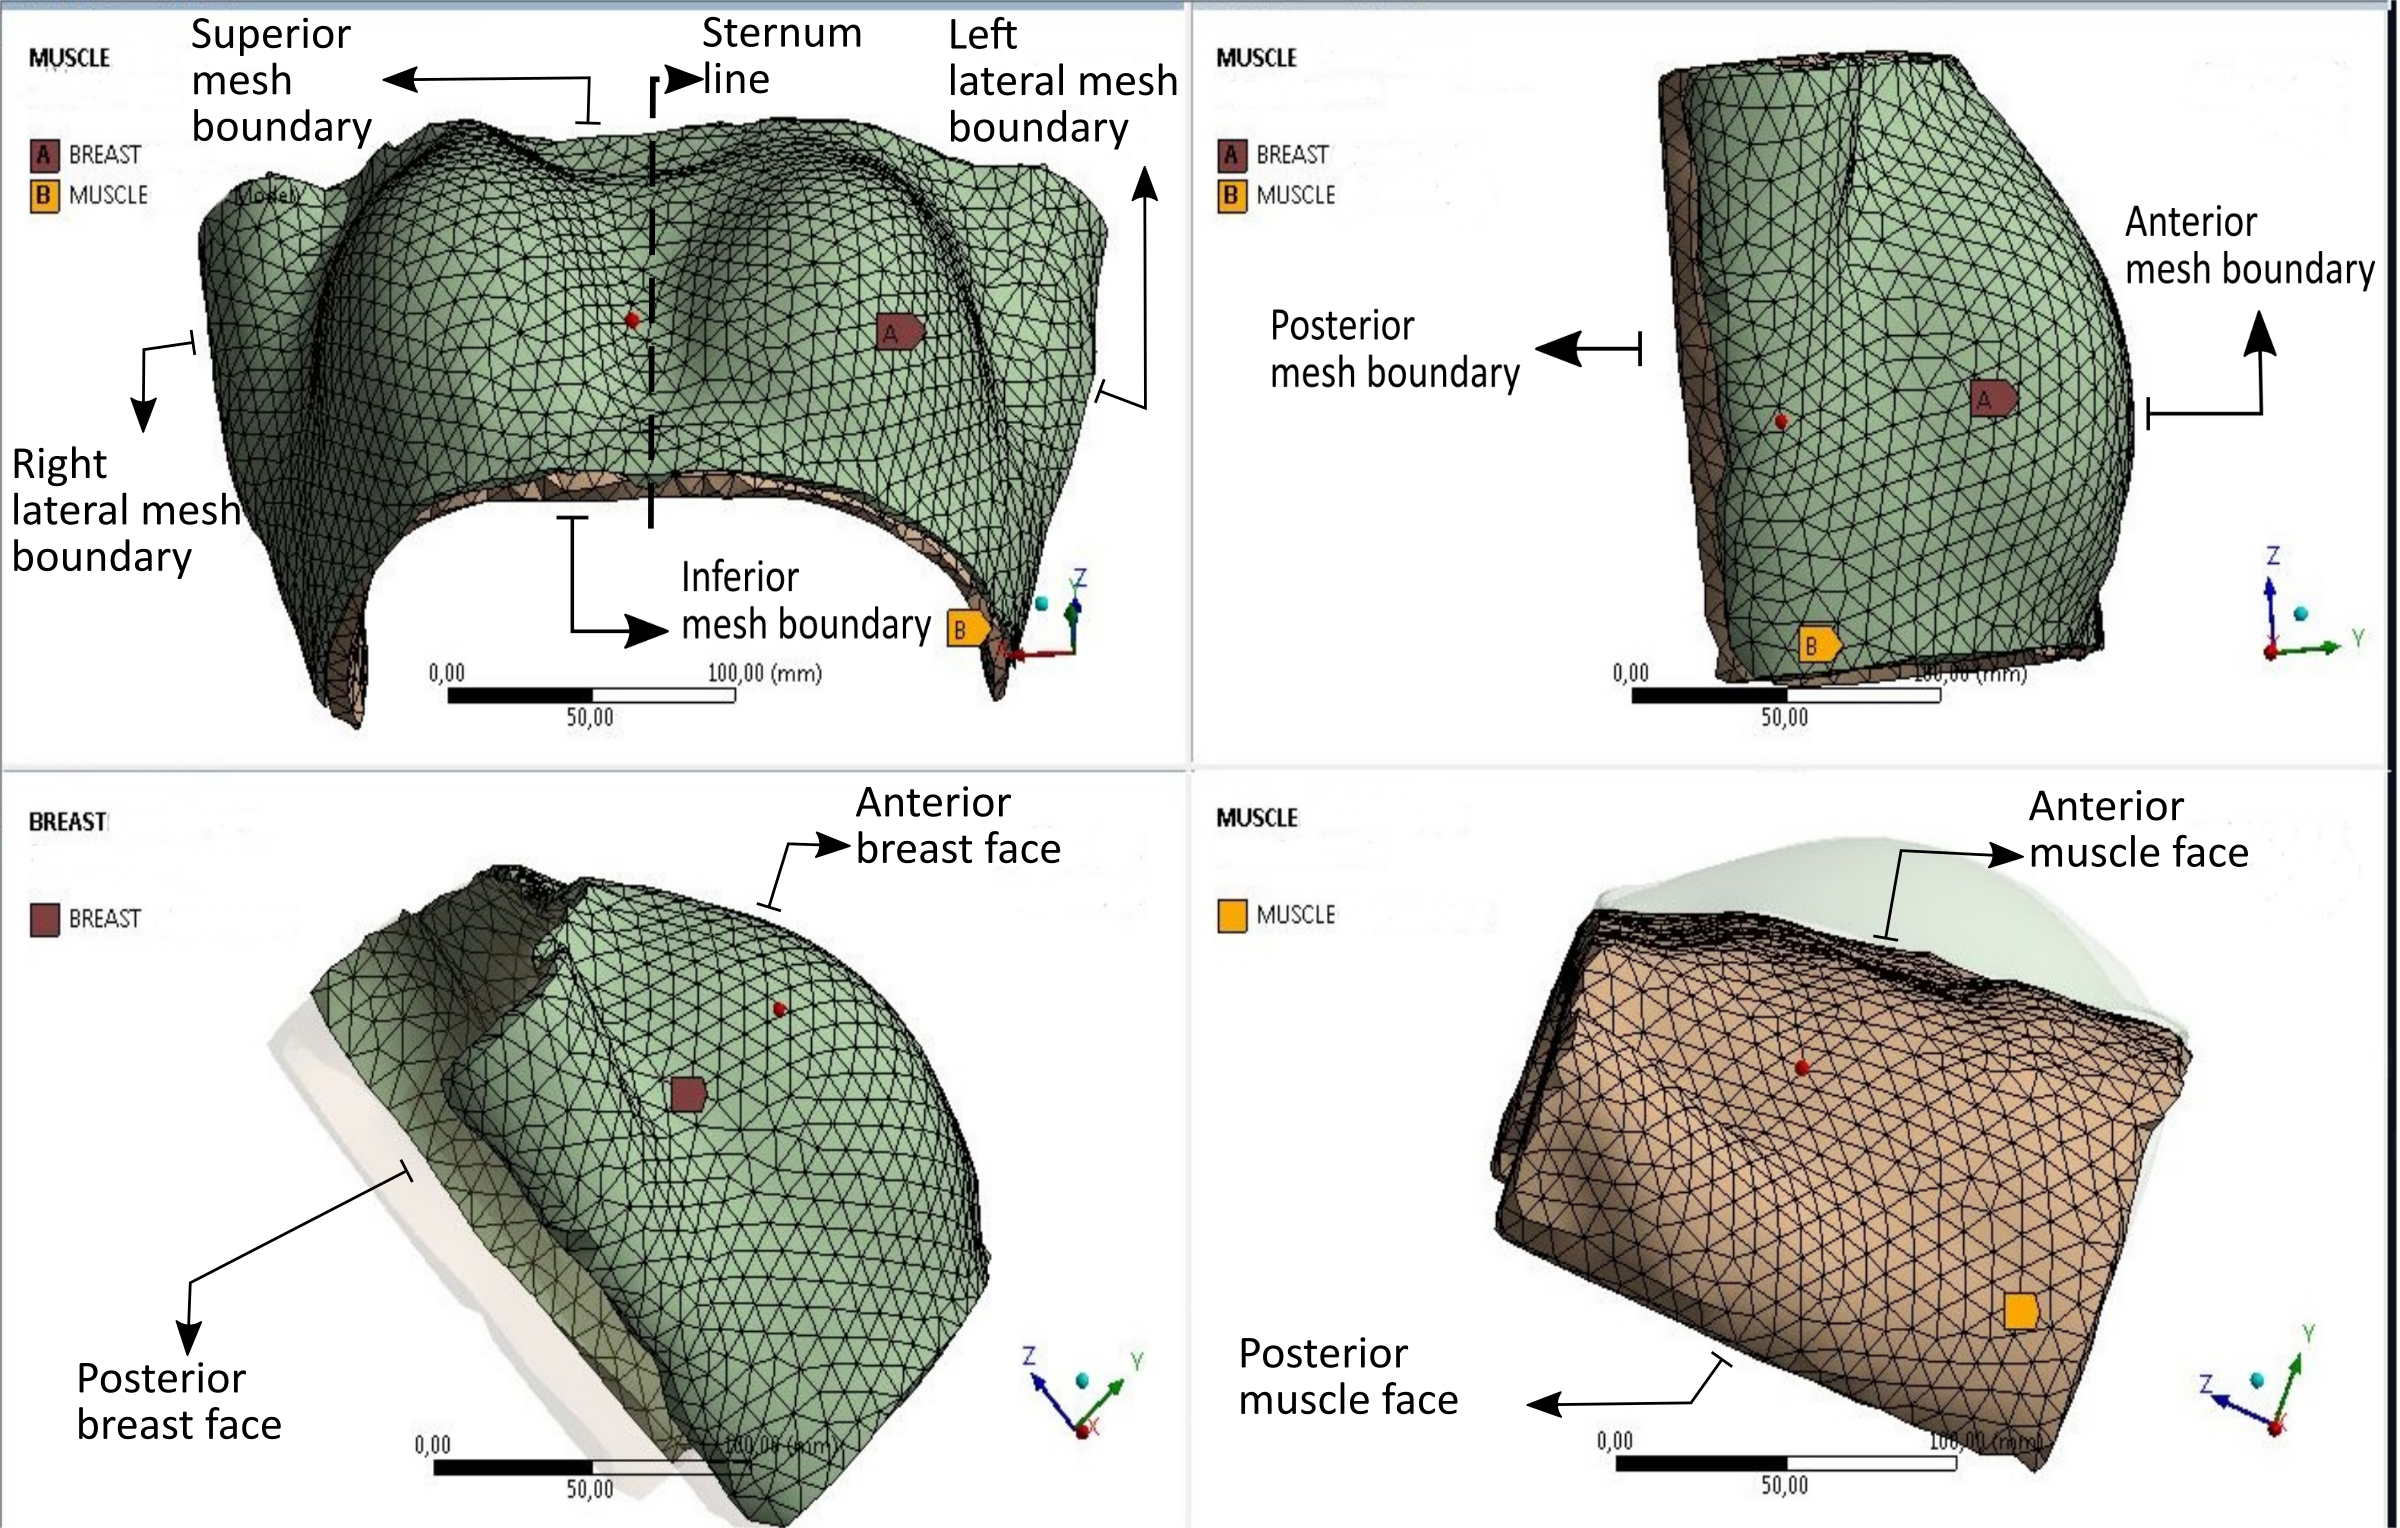
\includegraphics[width=0.9\textwidth,keepaspectratio]{figures/mesh_parts_2.png} 
\caption{Finite elements mesh boundaries}\label{fig:meshboundaries}
\end{figure}

Previous works have shown that modeling breast deformations from prone to supine configurations requires to take into account breast tissues sliding over the chest wall \citep{carter_application_2012,han_nonlinear_2014}. Moreover, anatomical books \citep{mugea2014aesthetic,clemente2011anatomy}  describe that the breast soft tissues are firmly attached to the deep fascia via suspensory ligaments but can move freely over the pectoralis muscle.  Therefore, the juncture surface is modeled as a no-separation contact with a frictional behavior proposed by the ANSYS Contact Technologies (see Section \ref{subsection:surfaceinteractionmodels}). The penalty algorithm is used with a meticulous control of contact normal and opening stiffness parameters. Stiffness parameters don't have a physical meaning and have to be identified by \textit{trial and error} methods. Since these parameters are extremely sensitive to the underlying elements stiffness and to the local deformation direction, new values have to be identified for each new simulation case.    

To study the impact of the friction coefficient $\mu_f$ on tissues sliding, several simulations have been performed at different values of $\mu_f$. We found that, with the Coulomb friction law, even for a high value of $\mu_f$, the tissues sliding is overestimated when estimating the prone breast configuration. When simulating prone breast configuration from the supine one, the sliding overestimation results also in an unconvergent solution due to element distortion. At the contact surface, because of excessive sliding, the tissue accumulation in the region of the sternum line results in a sinuous surface (Figure \ref{fig:overslidingProblem}) ; the finite element mesh  undergo important distortions and the solution is compromised. Therefore, different strategies based on anatomical breast structures were investigated to limit the amount of sliding and to overcome solution instabilities (Annex 2). However, it seams that a small amount of friction improves the solution convergence capabilities (see \cite{ansys_contact_2017}); therefore the friction coefficient is kept to $\mu_f = 0.1$. 
\begin{figure}[!h]
\centering
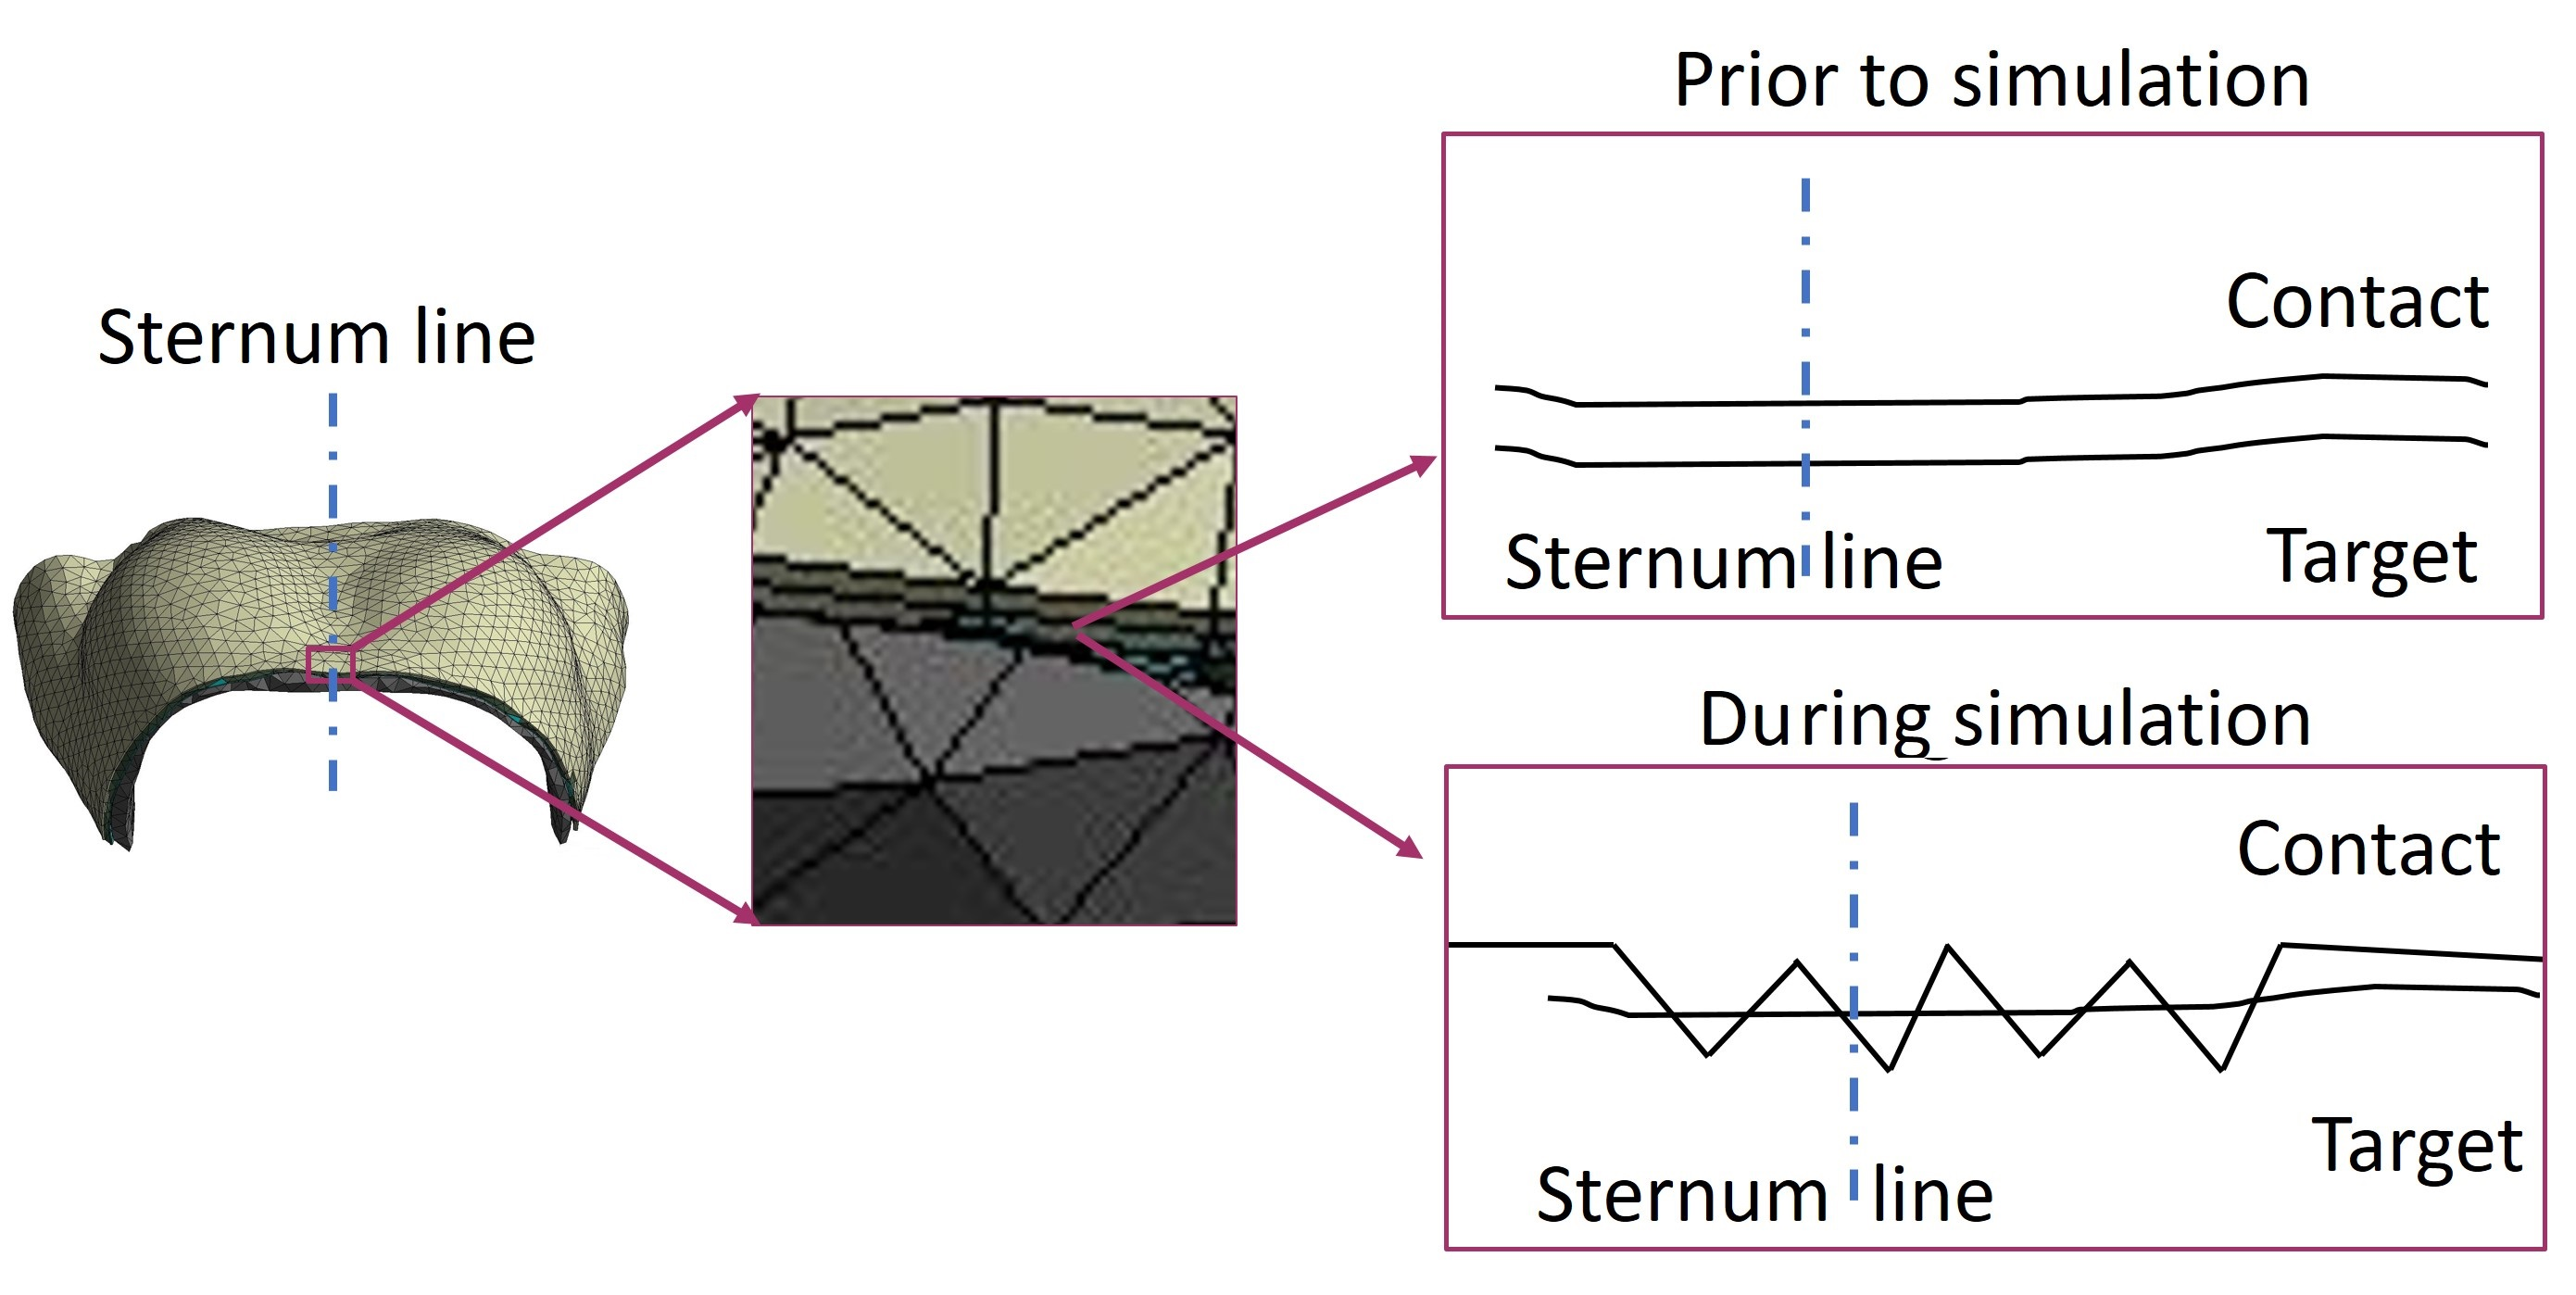
\includegraphics[width=0.7\textwidth,keepaspectratio]{figures/overslidingProblem.jpg} 
\caption{Tissues acumulation on the sternum line with excessive sliding}\label{fig:overslidingProblem}
\end{figure}
 
The strategy chosen to control the amount of tissues sliding relies on ligamentous breast structures described on Section \ref{subsection:internalstructures}. As concerns breast support matrix, only the largest structures are modeled, i.e. fascias and suspensory ligaments.  The superficial layer of superficial fascia is integrated in the skin layer, assuming a higher material stiffness. In addition, a new layer of 0.1mm thick shell elements is added at the juncture surface between muscle and breast tissue to model the deep layer of the superficial fascia. Shell elements and the underlying breast elements are sharing the same nodes. Since the deep fascia and muscle tissues are supposed to present similar elastic properties, the deep fascia is not explicitly modeled. In addition, two ligamentous structures (inframammary ligament and deep medial ligament) are modeled using Ansys link type elements connecting breast posterior surface nodes to anterior muscle surface nodes (Figure \ref{fig:mesh_components_BC}).  


Several additional Dirichlet conditions are set on the mesh boundaries: the superior and inferior ends of the deep fascia layer are constrained in Z direction; the superior and inferior ends of the skin layer are constrained in Y direction. For left and right lateral breast boundaries (Figure \ref{fig:meshboundaries}), Dirichlet conditions are too strong and preclude breast tissue to slide laterally. Therefore, in these regions new ligamentous structures are included with a cable-like behavior (Figure \ref{fig:mesh_components_BC}).



\begin{figure}[!h]
\centering
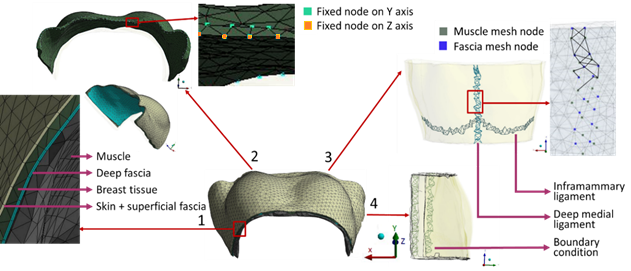
\includegraphics[width=0.9\textwidth,keepaspectratio]{figures/mesh_components.png} 
\caption{Components of the finite element mesh.}\label{fig:mesh_components_BC}
\end{figure}

 The deep layer of superficial fascia is much stiffer than the underlying adipose tissues. Due to imposed boundary conditions, the amount of sliding depends on fascia's elasticity. The suspensory ligaments define regions where the breast sliding is minimal regardless of the applied deformations. These additional stiff structures reduce the tissues sliding and improve the solution convergence capability. 

\section{Materials constitutive models}
\label{section:myConstitutivModels}

The final model consists of 6 types of tissues, wherein 4 tissues (glandular, fatty, muscle and skin) are well described and regularly used for biomechanical modeling and 2 of them (fascia and suspension ligaments) are with limited use and poorly described in the literature. A large range of constitutive parameters are available for each tissue. However because of an inconsistent interindividual variability, patient-specific parameters have to be identified.  


 Here, all materials except the suspensory ligaments are modeled using the Neo-Hookean strain energy. Breast suspensory ligaments are assumed to undergo only small deformations, thus they are considered as linear materials.  Patient-specific mechanical tissue properties are computed using an optimization process based on a multi-gravity loading simulation procedure (Figure \ref{fig:optimizationalgo}). First, for a given set of parameters $(\lambda_{glandular}$\nomenclature{$\lambda_{xx}$}{Youngs's moduli of the material $xx$}, $\lambda_{adipose}$, $ \lambda_{muscle}$,  $\lambda_{skin}$, $\lambda_{fascia}$, $\lambda_{ligam}$, $\nu$ ) the stress-free configuration is estimated by minimizing the difference between the simulated and the measured breast geometry in prone configuration. Then, from the new estimated stress-free geometry, the supine breast configuration is derived. The estimated supine geometry is compared to the measured one using modified Hausdorff distance, thus representing the estimation error.  To avoid taking into account the geometry dissimilarity due to arms position, the modified Hausdorff distance is computed only on breast skin surface.  
The process implies multiple simulation based on imposed nodes displacement; therefore the FE mesh can be significantly altered (with convergence issues) before reaching an optimal stress-free geometry. Mainly for that reason, we chose to perform an exhaustive manual rather than an automatic research of the optimal set of constitutive parameters. 


\begin{figure}[!h]
\centering
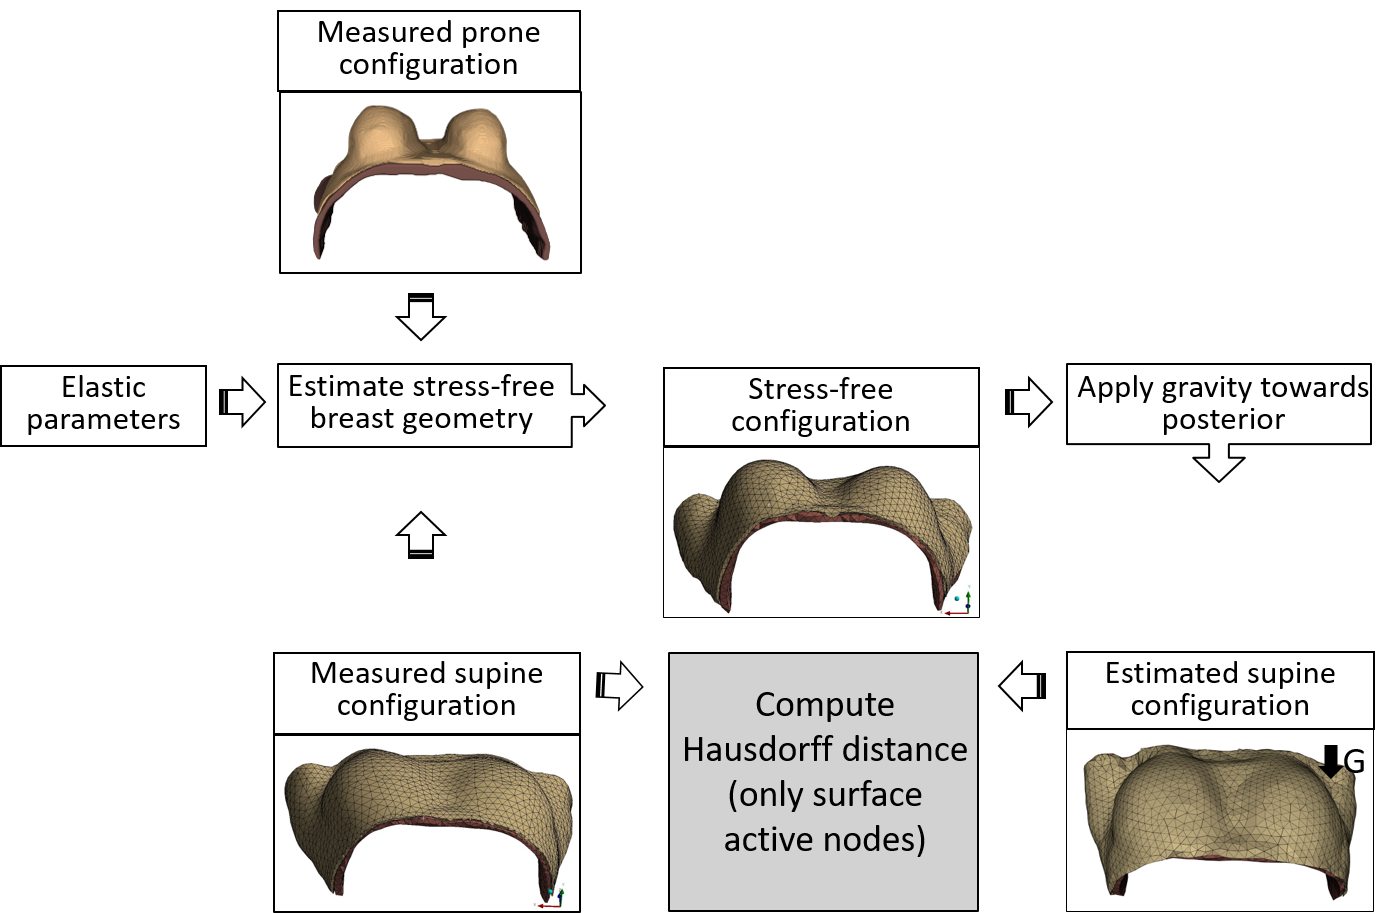
\includegraphics[width=0.9\textwidth,keepaspectratio]{figures/optimizationMaterialParameters.png} 
\caption{Process to estimate optimal material parameters}\label{fig:optimizationalgo}
\end{figure}
 
 An optimization process including finite element simulations with 6 parameters results is a complex and time-consuming problem. The model simplification is then performed in two steps. First, the parameters which variations have non-significant effects on simulation results are identified and set to an optimal fixed value. Next, for parameters which variations have a high impact, a sensitivity study is performed to redefine the search intervals and interval's discretization step.
 
 \subsection{Model simplification}

The breast tissues are mainly composed of water; a usual assumption is to consider them as nearly incompressible materials \citep{fung_biomechanics_2013}. However,
previous works proposed a Poisson's ratio value ranging between $\nu = 0.3$ \citep{hopp_automatic_2013} and $\nu = 0.5$ \citep{gamage_modelling_2012}. In a multi-loading gravity simulation, the breast volume is nearly constant, thus, the influence of Poisson's ratio on nodes displacements is studied only for values laying between $\nu = [0.45 , 0.495]$ (Figure \ref{fig:poissonRatio}). 

\begin{figure}[!h]
\centering
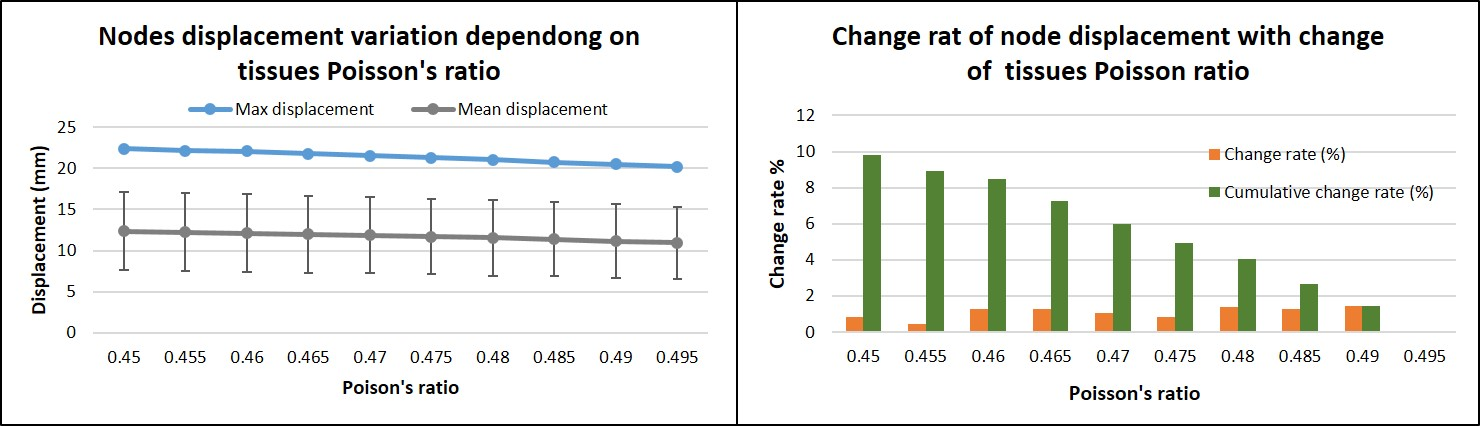
\includegraphics[width=\textwidth,keepaspectratio]{figures/poissonRatio.jpg} 
\caption{Process to estimate optimal material parameters}\label{fig:poissonRatio}
\end{figure}

The simulations were performed by applying the gravity force in posterio-anterior direction on breast geometry from supine configuration. On the right-hand side (Figure \ref{fig:poissonRatio}), the mean and the maximal displacements of the skin nodes are given for each values of $\nu$. On the left-hand side of the figure, the maximal difference of nodal displacements between two consecutive simulations (change rate) and the maximal difference of node displacements between the actual and the less deformed geometry (cumulative change rate) are plotted. The change rate is computed within the assumption that the maximal displacement over the simulations set represents 100\% change rate. Non-significant variations are observed on the mean and maximal displacements of skin nodes, thus a constant value of $\nu = 0.49$ was chosen.


The pectoral muscle together with the thoracic cage are the breast tissues support. The deformation of the muscle under gravity loading is neglected. Therefore, its Young's modulus was not included on the parametric study and was chosen so that only minimal deformations occur ($\lambda_{muscle}=10kPa$).

The ligamentous breast structures are added with a cable-like behavior to reduce tissues sliding. Their Young's modulus is also not included in the optimization process and is set sufficiently high ($\lambda_{ligam}=500kPa$) to preclude their elastic deformation. 

The adipose and glandular tissues are known to be extremely soft and to undergo large deformations under gravity loading.  \cite{calvo_polynomial_2015} proposed a uniform polynomial material model for the mixture of adipose and glandular tissues. The authors have also shown that the breast outer shape deformation does not depend on glandular distribution but is highly dependent on its volumetric ratio. It was also chosen here to model the glandular and fatty tissues as a single homogeneous material with an equivalent Young's modulus $\lambda_{breast }$. The mechanical properties of the equivalent breast tissue are in direct relation with glandular and adipose volumes ratios. Because the left and right breasts may have different granularities, two different parameters are considered ($\lambda_{breast}^l$ \nomenclature{$\lambda_{xx}^{l/r}$}{Young's modulus of the material xx for the left/right breast}, $\lambda_{breast}^r$).

Breast skin and superficial fascia are an essential part of the breast support matrix. The two layers are much stiffer than breast tissues and are the structures governing the amount of deformations. Their elastic behavior was included on the optimization process.

 Based on existing publications, an interval of possible values are given in Table \ref{table:minandmaxelasticmodulus} for each parameter included in the optimization process $(\lambda_{breast}^l$, $\lambda_{breast}^l$, $\lambda_{skin}$, $\lambda_{fascia})$. To characterize model sensitivity to parameters variations, a set of simulations were performed. The defined interval was discretized by steps of 10\% and at each step the skin nodes displacement were computed. Results of the corresponding simulations are shown on Figure  \ref{fig:materialPropDiscretization}. As previously, the first column represents the variation of mean and maximal displacements of skin nodes in function of the elastic parameter of each material; the second column represents the change rate and the cumulative change rate of skin nodes displacements.


\begin{table}[!h]
\centering
\begin{tabular}{|c||c|c|c||c|c|c|}
\hline
&\multicolumn{3}{|c||}{Search intervals}& \multicolumn{3}{c|}{Search intervals}\\
&\multicolumn{3}{|c||}{ from bibliographic data}& \multicolumn{3}{c|}{ after model simplification}\\
\hline
\hline
& Breast & Skin & Fascia & Breast & Skin & Fascia \\
\hline
Min (kPa)  & 0.3 & 7.4 & 100 & 0.3 & 2 & 50\\
\hline
Max (kPa) & 6 & 58.4 & 5000& 4& 20 &250 \\
\hline
\end{tabular}
\caption{Minimal and maximal value (in kPa) for Young's moduli.}
\label{table:minandmaxelasticmodulus}
\end{table}

The figure shows that the model is very sensitive to the variation of Young’s modulus of breast tissue, skin and fascia (Figure \ref{fig:materialPropDiscretization}). However, beyond some values, the materials become too stiff and do not change significantly the breast deformations under gravity loadings.  Therefore, the search intervals for breast tissue and skin Young's moduli are reduced so that a larger value impacts the cumulative change rate less than 20\% (max displacement less than $\sim 5mm$). As the fascia stiffness governs the lateral displacement and shows a smaller variation over the search interval, a threshold of 10 \% ($\sim 2.5mm)$ is chosen. The obtained search intervals are summarized in Table \ref{table:minandmaxelasticmodulus} 

\begin{figure}[!h]
\centering
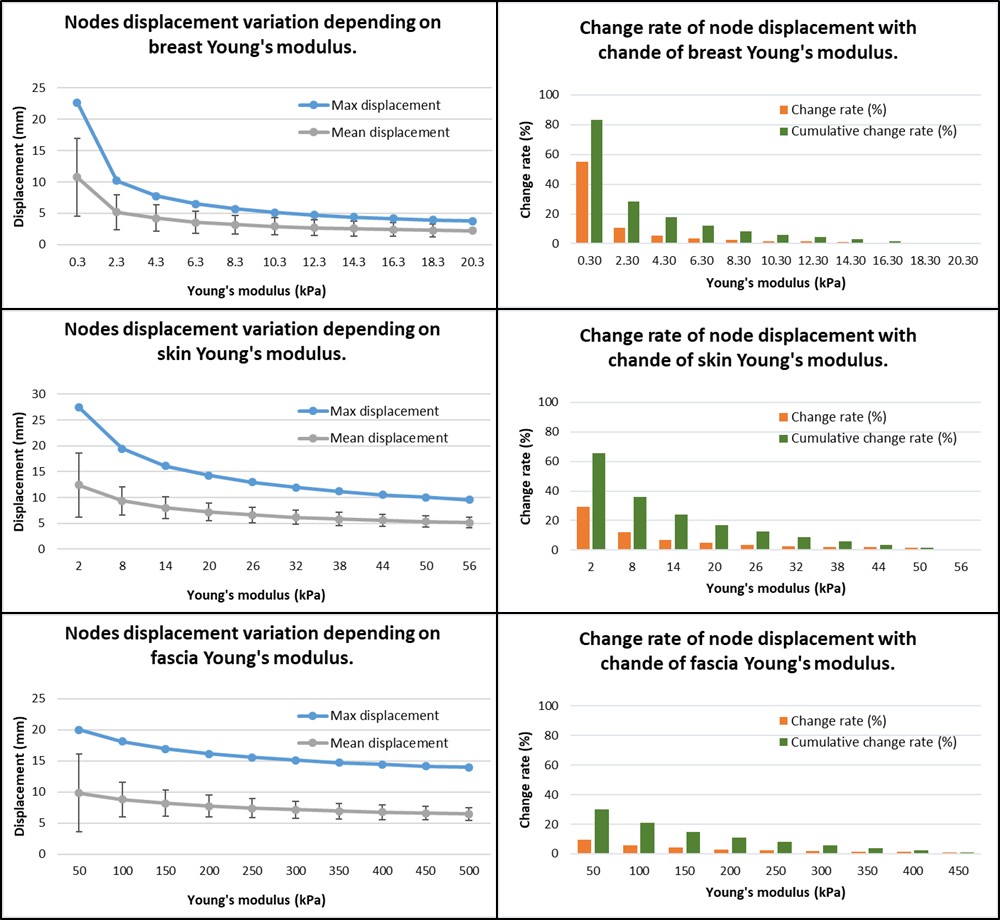
\includegraphics[width=\textwidth,keepaspectratio]{figures/materialPropDiscretization.png} 
\caption{First column: relation between maximal and mean nodes displacement and the equivalent Young's moduli variation for different tissues. Second column: rate and cumulative change rate of node displacement in function of quivalent Young's modulus}\label{fig:materialPropDiscretization}
\end{figure}

\subsection{Estimation of the optimal constitutive parameters}
To perform the optimization process, the new intervals defined by the above sensitive analysis are discretized by steps of $0.1 kPa$, $1kPa$ and $40 kPa$ respectively for breast, skin and fascia tissues. The discretization step is chosen such that the change rate between two consecutive simulations is less than 10\%.

The previously described multi-loading gravity process was performed for each parameters set and the corresponding model error distribution is shown in  Figure \ref{fig:optimizationresults}. The contour lines are estimated by linear interpolation between two consecutive simulations.

\begin{figure}[!h]
\centering
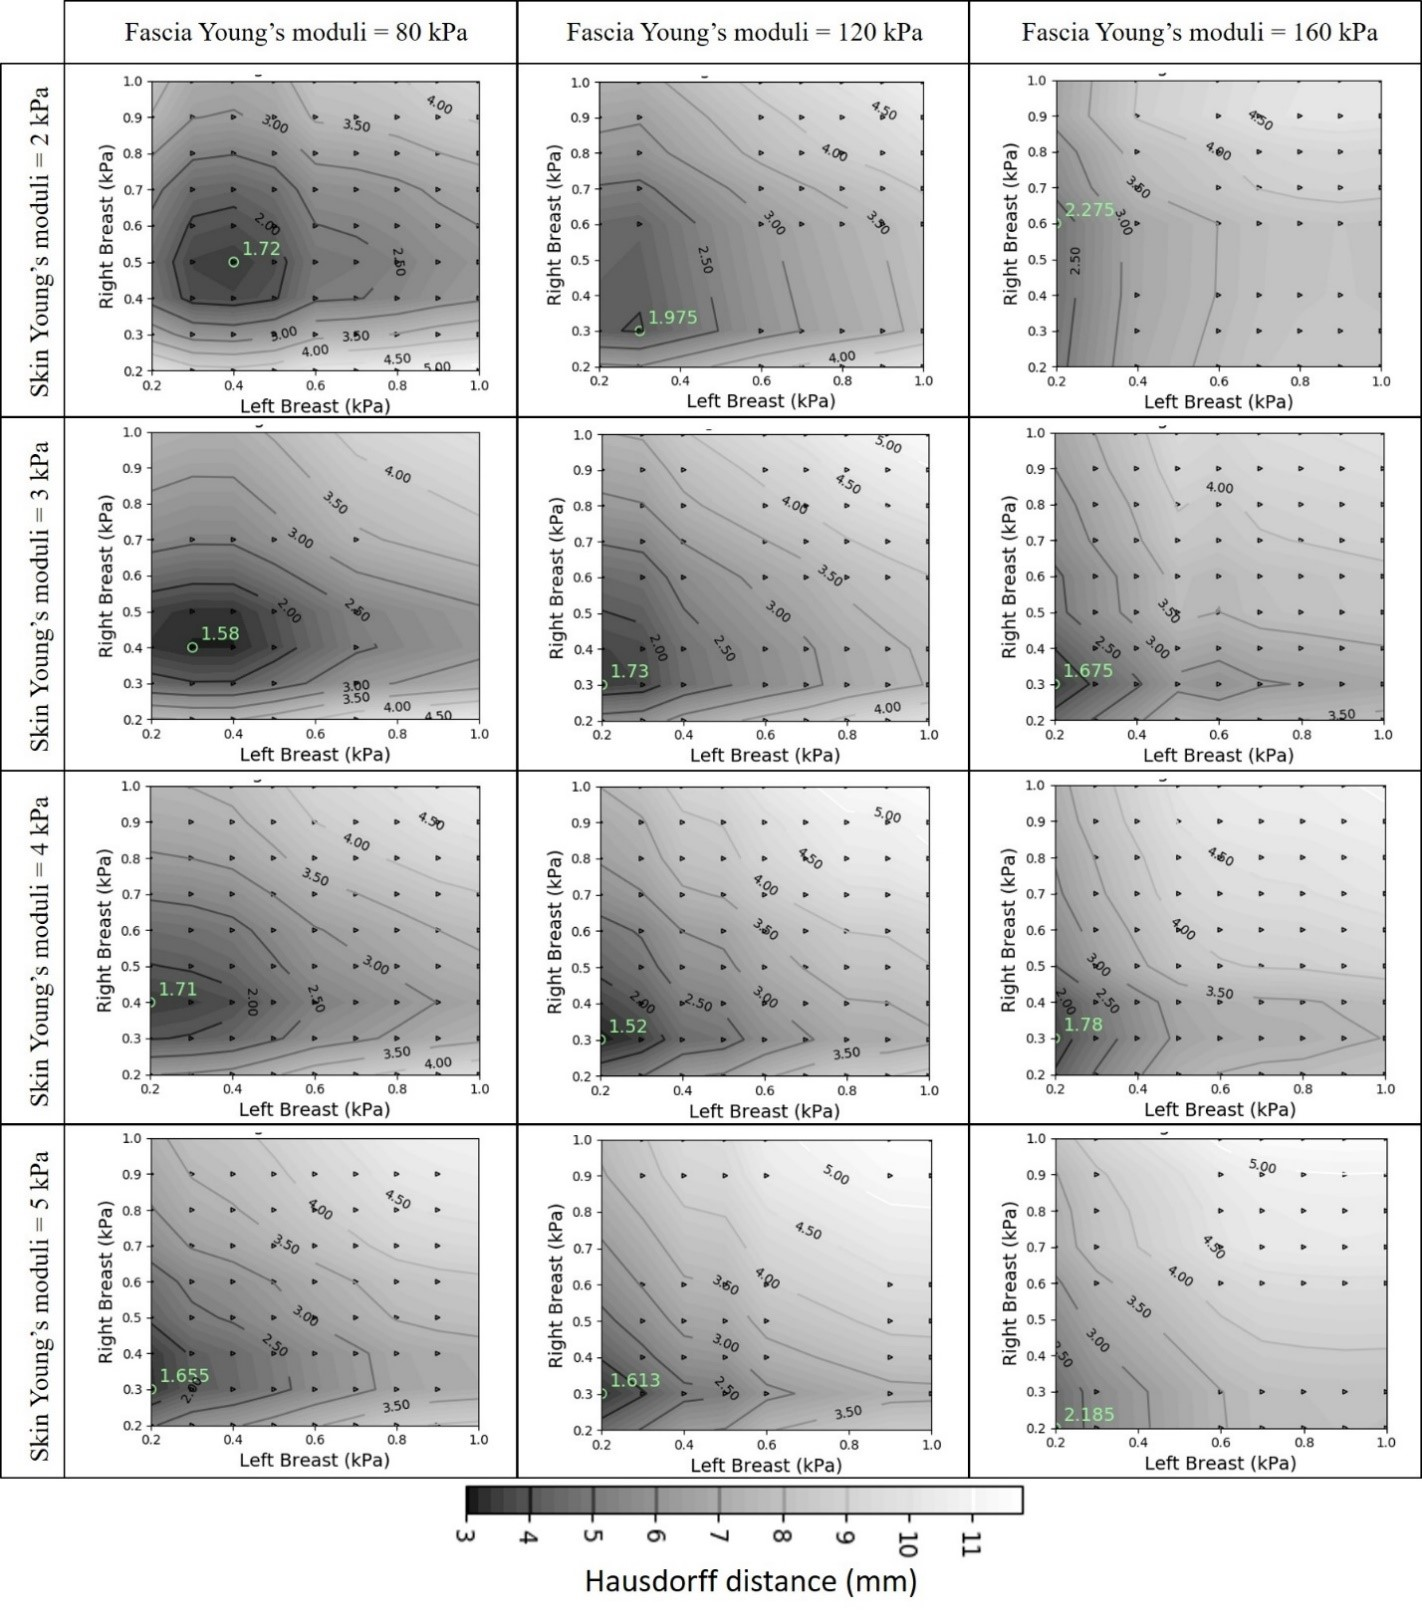
\includegraphics[width=0.9\textwidth,keepaspectratio]{figures/optimizationMaterialParameters2.png} 
\caption{Hausdorff distance on the skin surface over the constitutive parameters space}\label{fig:optimizationresults}
\end{figure}

It was found that the breast tissues Young's modulus is lower than the ones proposed in the bibliography, therefore more simulations were done outside the defined intervals. However, for very low values, below 0.2 kPa, 2 kPa and 80 kPa for breast, skin and fascia's Young's moduli respectively, the tissues deformation is too large and the finite element mesh becomes degenerated at the first step of the multi-loading simulation. For values above 1 kPa, 5 kPa and 160 kPa, tissues deformation is too small compared to the ones measured on the MR images and the simulations were excluded. All other missing values correspond to failed simulations due to a non-converging force, specifically in the region of the contact surface between the breast and the muscle.


 

For soft fascia ($\lambda_{fascia} = 80kPa$), the lateral displacement of breast tissues is more important than the one measured on MR images. Contrary, for stiff fascia material ($\lambda_{fascia}=160 kPa$) the amount of sliding is too small. To match the breast geometry in supine configuration, very low values for Young modulus are required ( $\lambda_{breast}< 0.2kPa$). For such low values, the breast tissues are highly deformed, thus the elements undergo distortions. Because of such errors in elements formulation the simulations giving the minimal Hausdorff distance have not succeeded.   

The set of parameters giving the best match between simulated and measured supine breast configurations is ($\lambda_{breast}^r=0.3 kPa$, $\lambda_{breast}^l=0.2 kPa$, $\lambda_{skin}=4 kPa$, $\lambda_{fascia}=120 kPa$).  

Figure \ref{fig:optimizationresults} shows the differences between the measured and estimated breast geometries in prone(left) and supine(right) configurations . Each distance was computed over the skin active nodes used also for the model optimization. 

\begin{figure}[!h]
\centering
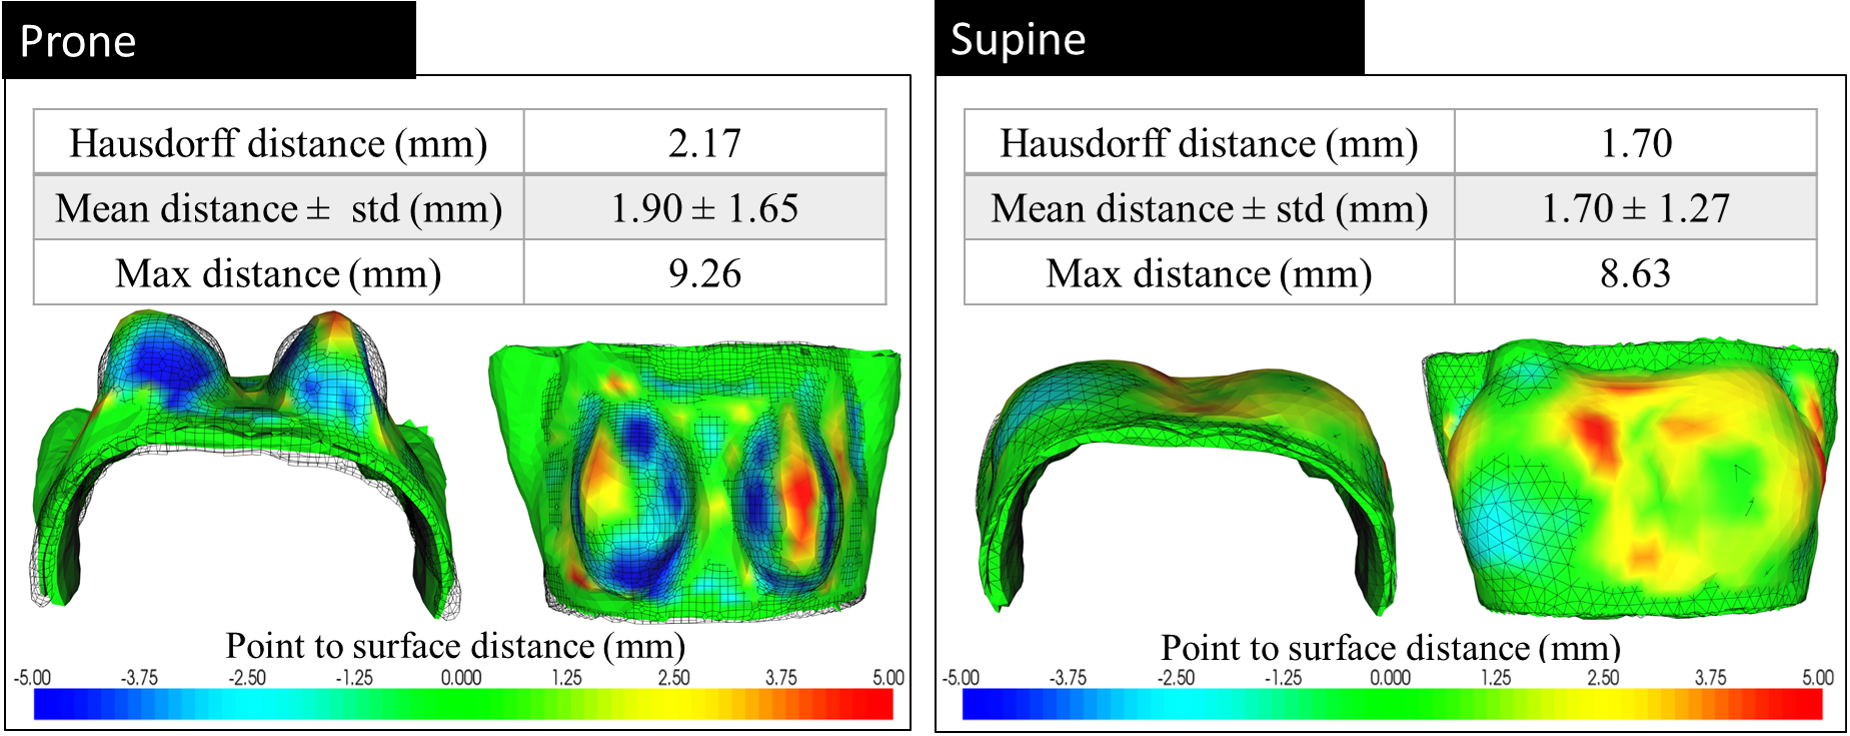
\includegraphics[width=\textwidth,keepaspectratio]{figures/optimizationresults.png} 
\caption{Difference  between estimated and measured data, in prone and supine geometries, obtained with optimal Young's moduli and stress-free geometry. }\label{fig:optimizationresults}
\end{figure}

The breast geometry is better estimated in supine configuration with an Hausdorff distance equal to 1.72 mm. This is probably due to a better representation of the boundary conditions in supine configuration, as this configuration was used to create the initial finite element mesh. The breast geometry in prone configuration is also well estimated with a modified Hausdorff distance equal to 2.17 mm. The maximal node to surface distance is obtained on the breast lateral parts.  Considering a non uniform skin thickness or elastic properties over the breast surface as described by \cite{sutradhar_vivo_2013} should improve the obtained results in prone configuration. 




